\chapter{Brief on quantitative finance}
This chapter is a very brief introduction to quantitative finance, more precisely, a collection of definitions concerning the financial markets which relate to the quantitative finance. The content of this chapter is based heavily on \cite{pw_iqf2ed_2007, ch_ofd9ed_2015}.


\section{Products and markets}
\subsection{Equities}
The most basic of financial instruments is the  \textbf{equity}\index{equity}, \textbf{stock}\index{stock} or \textbf{share}\index{share}. This is the ownership of a small piece of a company. Shares can be bought and sold freely on a regulated stock exchanges and capital can be raised efficiently. The behavior of the stock prices is far from being predictable because the prices have a large element of randomness. Therefore, the modeling must be done in a probabilistic sense. 

The value in holding stocks comes from the \textbf{dividends}\index{dividends} and any growth in the stock's value. Dividends are lump sum payments, paid out every quarter or every six months, to the holder of stock. The amount of the dividend varies depending on the profitability of the company. When the stock is bought, it either comes with its entitlement to the next dividends (\textbf{cum}\index{cum-dividend}) or not (\textbf{ex}\index{ex-dividend}). 

A stock is normally announced in a \textbf{stock-split}\index{stock-split}, e.g. a company with a stock price of \$90 announces a three-for-one split which simply means that instead of holding one stock valued at \$90, one holds three valued at \$30 each.
 
 
\subsection{Commodities}
Commodities are usually raw products such as precious metals, oil, etc. The prices of these products are unpredictable but often show seasonal effects. Commodities are usually traded by people who have no need of the raw material. Most trading is done on the futures market, making deals to buy or sell the commodity at some time in the future. The deal is then closed out before the commodity is due to be delivered. Futures contracts are discussed later.


\subsection{Currencies}
Countries in the world use different currencies, the rate at which one currency can be exchanged for another is the \textbf{exchange rate}\index{exchange rate}. This is the world of \textbf{foreign exchange}\index{foreign exchange}, or \textbf{Forex}\index{Forex} or \textbf{FX}\index{FX} for short. Whatever the exchange rates from one currency to another, there must be consistency throughout; otherwise it is possible to make \textbf{arbitrage profits}\index{arbitrage profits} by exploiting the mispricing.


\subsection{Indices}
For measuring how the stock market/economy is doing as whole, the stock market \textbf{indices}\index{indices} have been developed. A typical \textbf{index}\index{index} is made up from the weighted sum of a selection or \textbf{basket}\index{basket} of representative stocks. The selection may be designed to represent the whole market, such as the S\&P500 in the US or the FTSE100 in the UK, or a very special part of a market


\subsection{The time value of money}
The most fundamental concept in finance is the \textbf{time value of money}\index{time value of money}. \$100 today is worth more than \$100 in a year because of all the things we can do with \$100 over the year. You can lend the money to someone who can invest it in various risky ways (e.g. banks) and give you back the money with a little bit extra, the \textbf{interest}\index{interest}.

Let's denote the interest rates by $r$ and assume, for the moment, that $r$ are constant. Two most basic types of interest are simple and \textbf{compound}\index{compound}. Simple interest is when the interest is based only on the initial amount, whereas compound interest is when the interest has interest also. In reality, compound interest is the only case of relevance. Compound interest has two forms, \textbf{discretely compounded}\index{discretely compounded} and \textbf{continuously compounded}\index{continuously compounded}. The difference of these two types are illustrated below. 

\begin{center}
\begin{footnotesize}
\fbox{
\begin{minipage}{0.90\textwidth}
Suppose we invest \$100 in a bank at a discrete interest rate of $r$ paid \textit{once per annum}. After one year, the money becomes:
\begin{equation}
    100 \times \left( 1 + r \right)
\end{equation} 
and after $n$ years, we have:
\begin{equation}
    100 \times \left( 1 + r \right)^n
\end{equation}

Now, suppose there are $m$ interest payments at a rate of $r/m$ \textit{per annum}. After one year, the money in the bank is:
\begin{equation}
    100 \times \left( 1 + \frac{r}{m} \right)^m
\end{equation} 
Imagine that the interest payments come at increasingly frequent intervals, but at an increasingly smaller interest rate, this will lead to a rate of interest that is paid continuously. After one year, the money in the bank is:
\begin{equation}
    \lim_{m \to \infty}{100 \times \left( 1 + \frac{r}{m} \right)^m} \sim 100 \times e^r
\end{equation} 
And similarly, after $t$ years, we will have the amount:
\begin{equation}
    100 \times \left( 1 + \frac{r}{m} \right)^{mt} \sim 100 \times e^{rt}
    \label{cont_comp}
\end{equation} 

Equation \ref{cont_comp} can be derived via a differential equation. Suppose we have an amount $M(t)$ in the bank at time $t$. A short while later, time $t + dt$, the amount will have increased by:
\begin{equation}
    M(t+dt) - M(t) \approx \frac{dM}{dt}dt + \cdots 
\end{equation} 
where the rhs is a Taylor polynomial approximation. On the other hand, the interest we receive must be proportional to the amount we have $M$, the interest rate $r$ and the time step $dt$. Therefore:
\begin{equation}
    \frac{dM}{dt}dt = r \times M(t) dt \to \frac{dM}{dt} = r \times M(t)
\end{equation} 
This is the ordinary differential equation with the solution:
\begin{equation}
    M(t) = M(0) \times e^{rt}
\end{equation} 

The interest rate presented above is an important factor to relate the \textbf{present value}\index{present value}, $M(t)$, with the \textbf{future value}\index{future value}, $M(T)$, of the money as follows:
\begin{equation}
    M(t) = M(T) \times e^{-r(T-t)}
\end{equation} 
\end{minipage}
}
\end{footnotesize}
\end{center}


\subsection{Fixed-income securities}
A \textbf{fixed-income security}\index{fixed-income security} is an investment that provides a return in the form of \textbf{fixed periodic interest payments}\index{fixed periodic interest payment} and the eventual return of \textbf{principal at maturity}\index{principal at maturity}. Unlike \textbf{variable-income securities}\index{variable-income security}, where payments change based on some underlying measure — such as \textbf{short-term interest rates} or \textbf{floating interest rates}\index{floating interest payment} — the payments of a fixed-income security are known in advance. \textbf{Interest rate swaps}\index{interest rate swaps} are an exchange of a fixed rate of interest for a floating rate of interest.

There are various types of fixed income securities, such as:

\begin{itemize}
    \setlength\itemsep{0em}
    \item Bonds (both corporate and government) - the most common form of fixed-income securities;
    \item Treasury Bills;
    \item Money market instruments;
    \item Asset-backed securities.
\end{itemize}

The \textbf{index-linked bond}\index{index-linked bond} has been in the UK since 1981 and have provided a successful way to ensuring that income is not eroded by inflation (an inflation-proof bond). In the UK inflation is measured by the \href{https://www.investopedia.com/terms/r/rpi.asp}{\textbf{Retail Price Index (RPI)}}\index{Retail Price Index}; in the US the inflation index is the \href{https://www.investopedia.com/terms/c/consumerpriceindex.asp}{\textbf{Consumer Price Index (CPI)}}\index{Consumer Price Index}. The dynamics of the relationship between inflation and short-term interest rates is particularly interesting; the level of interest rates will affect the rate of inflation, but also interest rates are often used by central banks as a tool for keeping inflation down.


\subsection{Forwards and futures}
A \href{https://en.wikipedia.org/wiki/Forward_contract}{\textbf{forward contract}}\index{forward contract} is a private agreement between two parties giving the buyer an obligation to purchase an asset (and the seller an obligation to sell an asset) at a specified price (\textbf{the delivery price}\index{delivery price}) at a specified time (\textbf{the delivery date}\index{delivery date}) in the future. No money changes hands until the delivery date or \textbf{maturity}\index{maturity} of the contract. The asset could be a stock, a commodity or a currency. The \href{https://investinganswers.com/dictionary/f/forward-contract}{forward contract} has a value of zero initially. As we approach maturity, the value of the contract will change from initially zero to the difference between the underlying asset and the delivery price, at maturity.

A \href{https://en.wikipedia.org/wiki/Futures_contract}{\textbf{futures contract}}\index{futures contract} is very similar to a forward contract. \href{https://investinganswers.com/dictionary/f/futures-contract}{Futures contracts} are usually traded through an exchange, which standardizes the terms of the contracts - standardization means the same thing to everyone in the market. The profit or loss from the futures position is calculated every day and the change in this value is paid from one party to the other. Thus with futures contracts there is a gradual payment of funds from initiation until maturity. Because the change in value is settled on a daily basis, the value of a futures contract at any time during its life is zero. The different between the forward contracts and the future contracts can be found \href{https://en.wikipedia.org/wiki/Futures_contract}{here} or \href{https://www.investopedia.com/ask/answers/06/forwardsandfutures.asp}{here}. A series of brief lessons for forward and future contracts can be found \href{https://financetrain.com/series/futures-forwards/}{here}.

There are two kinds of forward- and future-contract participants: hedgers and speculators. Hedgers do not usually seek a profit but rather seek to stabilize the revenues or costs of their business operations; therefore hedging is avoidance of risk. Their gains or losses are usually offset to some degree by a corresponding loss or gain in the market for the underlying asset. Speculators are usually not interested in taking possession of the underlying assets. They essentially place bets on which way prices will go. 

Forward contracts tend to attract more hedgers than speculators. Speculators are often blamed for big price swings, but they also provide a lot of liquidity to the futures market. Look at section 1.9.1 in \cite{pw_iqf2ed_2007} for a hedged portfolio of asset and forward and the \textbf{no-arbitrage}\index{no-arbitrage} principle.

\begin{center}
\begin{footnotesize}
\fbox{
\begin{minipage}{0.90\textwidth}
Consider a forward contract that obliges us to hand over an amount \$$F$ at time $T$ to receive the underlying asset. Today's date is $t$ and the price of the asset is currently \$$S(t)$ - the \textbf{spot price}\index{spot price}. At maturity, we will hand over the amount \$$F$ and receive the asset then worth \$$S(T)$.

Assume that we simultaneously sell the asset when we enter into the forward contract - \textbf{going short}\index{going short} when we sell something we don't own. Now, we have an amount of $S(t)$ in cash due to the sale of the asset, a forward contract and a short asset position. Our net position now is zero. Then, we put the cash in the bank to receive interest. 
  
At maturity, we hand over the amount $F$ and receive the asset of $S(T)$ - this cancels our short asset position. We are also left with \textit{guaranteed} -$F$ in cash and the bank account with the initial investment of $S(t)$ with added interest. Our net position at maturity is then:
\begin{equation}
    S(t) \times e^{r(T-t)}-F
\end{equation}

Because we began with a portfolio worth zero and we end up with a predictable amount, that amount should also be zero (following the no-arbitrage principle). We can conclude that:
\begin{equation}
    F = S(t) \times e^{r(T-t)}
\end{equation}

This is the relationship between the spot price and the forward price. It is a linear relationship, the forward price is proportional to the spot price. If this relationship is violated then there will be an arbitrage opportunity. The standard economic argument then says that investors will act quickly to exploit the opportunity, and in the process prices will adjust to eliminate it.
\end{minipage}
}
\end{footnotesize}
\end{center}

Futures are usually traded publicly through an exchange which means they are very liquid
instruments and have lots of rules and regulations surrounding them. Here are a few
concepts related futures contracts.
\begin{itemize}
    \setlength\itemsep{0em}
    \item Available assets: a futures contract will specify the asset which is being invested in, the contract also specifies how many of each asset must be delivered, and the quantity will depend on the market. As an asset, a natural \href{https://en.wikipedia.org/wiki/Commodity}{\textbf{commodity}}\index{commodity} is particularly interesting because of non-uniformity in the type and quality of the asset to be delivered.
    \item Delivery and settlement: the futures contract will specify when the asset is to be delivered and settlement is the act of consummating the contract. The contract can be settled in \href{https://financetrain.com/settlement-of-futures-contracts/}{three ways}: (1) \textbf{closeout}\index{closeout}, (2) \textbf{physical delivery}\index{physical delivery} and (3) \textbf{cash settlement}\index{cash settlement}. Most futures contracts are closed out before delivery, with the trader taking the opposite position before maturity.
    \item Margin: changes in the value of futures contracts are settled each day - \textbf{marking to market}\index{marking to market}. To reduce the likelihood of one party defaulting, being unable or unwilling to pay up, the exchanges insist on traders depositing a sum of money to cover changes in the value of their positions. This money is deposited in a \textbf{margin account}\index{margin account}. Margin comes in two forms, the \textbf{initial margin}\index{initial margin} and the \textbf{maintenance margin}\index{maintenance margin}. The initial margin is the amount deposited at the initiation of the contract. The total amount held as margin must stay above a prescribed maintenance margin. If it ever falls below this level then more money (or equivalent in bonds, stocks, etc.) must be deposited. 
    \item Commodity futures: futures on commodities don't necessarily obey the no-arbitrage law that led to the asset/future price relationship because of the messy topic of storage. The holder of the futures contract must compensate the holder of the commodity for his storage costs. This can be expressed in percentage terms by an adjustment $s$ to the risk-free rate of interest. On the other hands, most people actually holding the commodity are benefiting from it in some way. And the benefit from holding the commodity is commonly measured in terms of the convenience yield $c$:
\begin{equation}
    F = S(t) \times e^{(r+s-c)(T-t)}
\end{equation}
Depending on the storage cost and the convenience yield, the price varies. When 
\begin{equation}
    F < S(t) \times e^{r(T-t)}
\end{equation}
the market is said to be \textbf{backwardation}\index{backwardation}; when 
\begin{equation}
    F > S(t) \times e^{r(T-t)}
\end{equation}
the market is said to be \textbf{contango}\index{contango}.
    \item FX futures: there are no problems associated with storage when the asset is a currency, we only need to modify the no-arbitrage result to allow for interest received on the foreign currency $r_f$. Then we have:
    \begin{equation}
    F = S(t) \times e^{(r-r_f)(T-t)}
\end{equation}
    \item Index futures: futures contracts on stock indices are settled in cash. Again, there are no storage problems, but now we have dividends, which play a role similar to that of a foreign interest rate on FX futures, to contend by the dividend yield $q$. 
\begin{equation}
    F = S(t) \times e^{(r-q)(T-t)}
\end{equation}
\end{itemize}

Here are the summary of a few loose definitions for the important financial terminologies that have been presented above. 
\begin{itemize}
    \setlength\itemsep{0em}
    \item \textbf{Premium}\index{premium}: the amount paid for the contract initially.
    \item \textbf{Underlying (asset)}\index{underlying asset} the financial instrument on which the option value depends denoted by $S$. The option payoff is defined as some function of the underlying asset at expiry.
    \item \textbf{Strike (price)} or \textbf{exercise price}: the amount for which the underlying can be bought (call) or sold (put) denoted by $E$. This definition only really applies to the simple calls and puts.
    \item \textbf{Expiration (date)} or \textbf{expiry (date)}: date on which the option can be exercised or date on which the option ceases to exist or give the holder any rights denoted by $T$.
    \item \textbf{Intrinsic value}\index{intrinsic value}: the payoff that would be received if the underlying is at its current level when the option expires.
    \item \textbf{Time value}\index{time value}: any value that the option has above its intrinsic value since the option value is generally different from the intrinsic value.
    \item \textbf{In the money}\index{in the money}: an option with positive intrinsic value. A call option when the asset price is above the strike, a put option when the asset price is below the strike.
    \item \textbf{Out of the money}\index{out of the money}: an option with no intrinsic value, only time value. A call option when the asset price is below the strike, a put option when the asset price is above the strike.
    \item \textbf{At the money}\index{at the money}: a call or put with a strike that is close to the current asset level.
    \item \textbf{Long position}\index{long position}: a positive amount of a quantity, or a positive exposure to a quantity.
    \item \textbf{Short position}\index{short position}: a negative amount of a quantity, or a negative exposure to a quantity. Many assets can be sold short, with some constraints on the length of time before they must be bought back. More explanation for the long and short position can be found \href{http://positron-investments.com/en/technical-analysis-basics/long-versus-short-selling/}{here}.
\end{itemize}


\section{Derivatives}
\subsection{Options}
In the future or forward contracts, the holder is obliged to trade at the maturity of the contract. The \textbf{option}\index{option} gives the holder the \textit{right} to trade in the future at a previously agreed price but takes away the obligation, e.g. if the stock falls, we don't have to buy it after all. A \textbf{call option}\index{call option} is the right to buy a particular asset for an agreed amount (the \textbf{exercise price}\index{exercise price} or \textbf{strike price}\index{strike price}) at a specified time in the future (the \textbf{expiry}\index{expiry} or \textbf{expiration date}\index{expiration date}). The stock on which the option is based is known as the \textbf{underlying asset}\index{underlying asset}. We would exercise the option at expiry if the stock is above the strike and not if it is below. If we use $S$ to mean the stock price and $E$ the strike then at expiry the option is worth:
\begin{equation}
    \max(S - E, 0)
\end{equation}
This function of the underlying asset is called the \textbf{payoff function}\index{payoff function}.

A \textbf{put option}\index{put option} is the right to sell a particular asset for an agreed amount at a specified time in the future. The holder of a put option wants the stock price to fall so that he can sell the asset for more than it is worth. The payoff function for a put option is:
\begin{equation}
    \max(E - S, 0)
\end{equation}
And now the option is only exercised if the stock falls below the strike price.

Calls and puts have a non-linear dependence on the underlying asset. The randomness in the underlying asset and the curvature of the option value with respect to the asset are intimately related. Other terms used to describe contracts with some dependence on a more fundamental asset are \textbf{derivatives}\index{derivatives} or \textbf{contingent claims}\index{contingent claim}.

An option's value at expiry is normally visualized in a \href{http://positron-investments.com/en/options-basics/payoff-diagrams/}{\textbf{payoff diagram}}\index{payoff diagram} in which the value of an option at expiry is a function of the underlying, or in a \textbf{profit diagram}\index{profit diagram} in which the payoff subtracted by the premium originally paid for the call option is a function of the underlying. More explanation on the loss/profit diagram can be found \href{https://www.optiontradingtips.com/options101/payoff-diagrams.html}{here}.

The \href{http://positron-investments.com/en/options-basics/option-buyer-vs-option-writer/}{\textbf{writer}}\index{writer} of an option is the person who promises to deliver the underlying asset, if the option is a call, or buy it, if the option is a put. The writer is the person who receives the premium. Writing options is very risky. The downside of buying an option is just the initial premium, the upside may be unlimited. The upside of writing an option is limited, but the downside could be huge. To cover the risk of default in the event of an unfavorable outcome, the \textbf{clearing houses}\index{clearing houses} that register and settle options insist on the deposit of a margin by the writers of options.

Most of the simpler options contracts are bought and sold through \textbf{exchanges}\index{exchange}. These exchanges make it simpler and more efficient to match buyers with sellers. Part of this simplification involves the conventions about features of the contracts. Having standardized contracts traded through an exchange promotes liquidity of the instruments. Some options are an agreement between two parties, often brought together by an intermediary. These agreements can be very flexible and the contract details do not need to satisfy any conventions. Such contracts are known as \textbf{over the counter}\index{over the counter} or \textbf{OTC}\index{OTC} contracts.


\subsection{The value of the option}
The \textit{fair value} of the option contracts $V$ depends on the underlying asset price $S$ and time $t$, $V(S,t)$. At the expiry date $t = T$, the function $V$ is the payoff function, e.g. for the call option:
\begin{equation}
    V(S,T) = \max(S - E, 0)
\end{equation}    

Factors influencing the derivative prices consists of \textbf{variables}\index{variables} (e.g. the value of the underlying asset $S$ and the time to expiry $t$) and \textbf{parameters}\index{parameters} (e.g. the interest rate and the strike price). There is one important parameter which has a major impact on the option value. That parameter is the \textbf{volatility}\index{volatility} which is a measure of the amount of fluctuation in the asset price, a measure of the randomness. Volatility is a particularly interesting parameter because it is so hard to estimate since it never stays constant and is unpredictable.


\subsection{Speculation and gearing}
If you buy a far out-of-the-money option it may not cost very much, especially if there is not very long until expiry. If the option expires worthless, then you also have not lost very much. However, if there is a dramatic move in the underlying, so that the option expires in the money, you may make a large profit relative to the amount of the investment. This is an example of \textbf{gearing}\index{gearing} or \textbf{leverage}\index{leverage}. The out-of-the-money option has a high gearing, a possible high payoff for a small investment. The downside of this \href{https://en.wikipedia.org/wiki/Leverage_(finance)}{leverage} is that the call option is more likely than not to expire completely worthless and you will lose all of your investment. Further reading about gearing and leverage can be found in \href{https://www.investopedia.com/terms/l/leverageratio.asp}{here}, \href{https://www.investopedia.com/terms/g/gearingratio.asp}{here} and \href{https://specialties.bayt.com/en/specialties/q/146664/what-is-the-difference-between-leverage-ratio-and-gearing-ratio/}{here}

Due to the unpredictable adverse price movements in an asset, the writer of the option normally buy other contracts to offset his risk. This offsetting of risk by buying other related contracts is called \textbf{hedging}\index{hedging}. \href{https://en.wikipedia.org/wiki/Hedge_(finance)}{Hedging} is the practice of taking a position in one market to offset and balance against the risk adopted by assuming a position in a contrary or opposing market or investment. Further reading about hedging can be found in \href{https://www.investopedia.com/terms/h/hedge.asp}{here} and \href{https://www.investopedia.com/trading/hedging-beginners-guide/}{here}.


\subsection{Option strategies}
\subsubsection{Single-option}
Calls and puts are the two simplest forms of option, they are often referred to as \textbf{vanilla}\index{vanilla}. Increasingly important are the \textbf{binary}\index{binary option} or \textbf{digital options}\index{digital option}. Binary options have an expiry date and/or time. At the time of expiry, the price of the underlying asset must be on the correct side of the strike price (based on the trade taken) for the trader to make a profit. Further explanations on the binary options can be found \href{https://www.investopedia.com/terms/b/binary-option.asp}{here}.

Three other popular options in practice are:
\begin{itemize}
    \setlength\itemsep{0em}
    \item \textbf{American options}\index{American option} which can be exercised at any time up to the maturity;
    \item \textbf{European options}\index{European option} which can be exercised only on the expiration date itself; and,
    \item \textbf{Bermudan options}\index{Bermudan option} which allow exercise on specified dates or in specified periods.
\end{itemize} 


\subsubsection{Put-Call parity}
Imagine that today at $t$ you buy one European call option with a strike of $E$ and an expiry of $T$ and that you write a European put option with the same strike and expiry, you now have a pair of long-call and short-put. The payoff for the portfolio of the two options is the sum of the individual payoffs:
\begin{equation}
    \max(S(T) - E, 0) - \max(E - S(T), 0) = S(T) - E
\end{equation}  
where $S(T)$ is the value of the underlying asset at time $T$, today it cost you $S(t)$. 

The cash-flow of the portfolio is independent of the future behaviour of the stock and is modelled as:
\begin{equation}
    C - P = S - Ee^{-r(T-t)}
\end{equation}  
where $C$ and $P$ are today's values of the call and the put respectively. This relationship holds at any time up to expiry and is known as the \textbf{put-call parity}\index{put-call parity}. If this relationship did not hold then there would be riskless arbitrage opportunities.
 

\subsubsection{Multiple-option}
In a portfolio, normally several different options are combined to maximize the profit or minimize the risk. There are numerous combinations in practice, a few simple one can be listed as:
\begin{itemize}
    \setlength\itemsep{0em}
    \item \href{https://www.investopedia.com/terms/s/spread.asp}{Spread}
    \item \href{https://www.investopedia.com/terms/b/bullspread.asp}{Bull spread}
    \item \href{https://www.investopedia.com/terms/b/bearspread.asp}{Bear spread}
    \item \href{https://www.investopedia.com/terms/c/condorspread.asp}{Condor spread}
    \item \href{https://www.investopedia.com/terms/c/calendarspread.asp}{Calendar spread}
    \item \href{https://www.investopedia.com/terms/c/creditspread.asp}{Credit spread}
    \item \href{https://www.investopedia.com/terms/d/debitspread.asp}{Debit spread}
    \item \href{https://brilliant.org/wiki/straddle-strangle/}{Straddle and Strangle} and \href{https://www.investopedia.com/ask/answers/05/052805.asp}{their differences}
    \item Risk reversal 
\end{itemize}


\subsubsection{Miscellaneous}
\begin{itemize}
    \setlength\itemsep{0em}
    \item \textbf{Warrants}\index{warrant}: a contract that is very similar to an option is a warrant.Warrants are call options issued by a company on its own equity. The main differences between traded options and warrants are the timescales involved, warrants usually have a longer lifespan, and on exercise the company issues new stock to the warrant holder. On exercise, the holder of a traded option receives stock that has already been issued.
    \item \textbf{Convertible bonds}\index{convertible bond}: convertible bonds (or \textbf{CBs}) have features of both bonds and warrants. They pay a stream of coupons with a final repayment of principal at maturity, but they can be converted into the underlying stock before expiry. Because the CB can be converted into the asset, its value has to be at least the value of the asset. This makes CBs similar to American options
    \item \textbf{Over-the-Counter (OTC)}\index{over-the-counter, OTC} options: Not all options are traded on an exchange. Some, known as over the counter or OTC options, are sold privately from one counter-party to another.
\end{itemize}



\section{The binomial model}
\label{sec:intro_binomial_model}
\subsection{Introduction}
The binomial model is the simplest model for asset prices that can be used for pricing derivatives and to explain a couple of very important financial concepts. The original binomial concept is due to Cox et al. \cite{cox_optionpricing_1979}. More details description of the model can be found in \cite{pw_poqf2ed_2006, pw_iqf2ed_2007, ch_ofd9ed_2015}. Hull \cite{ch_ofd9ed_2015} also describes its use in the fixed-income world. Mathematical treatment of the binomial model is briefly presented in Section \ref{sec:binomial_tree}. This section only summaries the main idea of the binomial model based on the illustration in Chapter 3 of \cite{pw_iqf2ed_2007}.

\begin{center}
\begin{footnotesize}
\fbox{
\begin{minipage}{0.90\textwidth}
The model is used for the behavior of an equity, e.g. a stock and to illustrate how to value options. The starting point of the model includes:
\begin{itemize}
    \setlength\itemsep{0em}
    \item We will have a stock currently worth \$100.
    \item The stock can either rise or fall by a known amount at a known probability between today and tomorrow; a rise to \$101 with a probability of 0.6 and a fall to \$99 with a probability of 0.4. 
    \item Interest rates are zero.
\end{itemize}

We have the call option on the stock with a strike of \$100 and expires tomorrow. The question is what the option is worth today ? Sadly, not \textbf{0.6} as you may calculate with the rise/fall amounts and the corresponding probability, but \textbf{0.5}. 

To understand the option value of 0.5, we must construct a portfolio consisting of one option and short $\frac{1}{2}$ of the underlying stock. By doing so, the portfolio takes the value of $-\frac{99}{2}$ regardless of whether the stock rises or falls. This portfolio is a perfectly \textbf{risk-free portfolio}\index{risk-free portfolio}. As the portfolio is worth $-\frac{99}{2}$ tomorrow and interest rates are zero, it must also be wroth $-\frac{99}{2}$ today. This is an example of \textbf{no arbitrage}\index{no arbitrage}. 

In the above example, the value of an option does not depend on the probability of the stock rising or falling. This is equivalent to saying that the stock growth rate is irrelevant for \href{https://www.investopedia.com/terms/o/optionpricingtheory.asp}{option pricing}. This is because we have \textbf{hedged} \textit{the option with the stock} hence we do not care whether the stock rises or falls.

The quantity of stock that much be sold for hedging is $\frac{1}{2}$. This is called as \textbf{Delta-hedging}\index{Delta-hedging}, $\Delta$, which means choosing a proportion such that the portfolio value does not depend on the direction of the stock. In general:
\begin{equation}
    \Delta = \frac{\text{range of option payoffs}}{\text{range of stock prices}} = \frac{1-0}{101-99} = \frac{1}{2}
\end{equation}
which actually comes from the equality:
\begin{equation}
    1 - \Delta \times 101 = 0 - \Delta \times 99
\end{equation}
$\Delta$ can represent the sensitivity of the option to changes in the stock.

How does the option value change if the interest rate is non-zero? We still delta-hedge as before to construct a risk-free portfolio, then we use exactly the same delta to present value that back in time by multiplying by a discount factor. 

Assume that $r = 0.1$ then the discount factor for going back one day is:
\begin{equation}
    \frac{1}{1+0.1/252} = 0.9996
\end{equation}

The portfolio value today must be the \textit{present value} of the portfolio value tomorrow:
\begin{equation}
    ? - 0.5 \times 100 = 0 - 0.5 \times 99 \times 0.9996
\end{equation}
so that $? = 0.51963$.
\end{minipage}
}
\end{footnotesize}
\end{center}

The \textbf{theoretical price}\index{theoretical price} derived above should be identical to the \textbf{market price}\index{market price} otherwise there is risk-free money to be made. If the option costs less than 0.5 simply buy it and hedge to make a profit. If it is worth more than 0.5 in the market then sell it and hedge, and make a guaranteed profit. In reality, it is possible for arbitrage opportunities to exist, and to exist for a long time. The market also really need there to be some practical mechanism for arbitrage to be `removed'. Supply and demand should act to make the option price converge to the 0.5.


\subsection{Risk-neutrality}
In the \textbf{real world}\index{real world}, statistical skills have been used to estimate the future possible stock prices (99 and 101) and the probabilities of reaching them (0.4 and 0.6). Some properties of the real world can be listed as (1) we know about delta hedging and risk elimination; (2) we are sensitive to risk and expect greater return for taking risk; and (3) only the two stock prices matter for option pricing, not the probabilities.

People often refer to the \textbf{\href{https://www.investopedia.com/terms/r/riskneutral.asp}{risk-neutral} world}\index{risk-neutral world} in which people don't care about risk. The risk-neutral world has the following characteristics (1) we don't care about risk, and don't expect any extra return for taking unnecessary risk; (2) we don't ever need statistics for estimating probabilities of events happening; and (3) we believe that everything is priced using \textbf{simple expectations}.

\begin{center}
\begin{footnotesize}
\fbox{
\begin{minipage}{0.90\textwidth}
Imagine that we are in the risk-neutral world and:
\begin{itemize}
    \setlength\itemsep{0em}
    \item we have a stock currently worth \$100;
    \item the stock can either rise to \$101 or fall to \$99. 
\end{itemize}

Using simple expectation and the symmetry of rising/falling, the \textbf{risk-neutral probability}\index{risk-neutral probability} $p'$ can be calculated from:
\begin{equation}
    p' \times 101 + (1-p') \times 99 = 100
\end{equation}
hence $p' = 0.5$. Please note that $p'$ is only a mathematical term, it is not real since it is derived based on a fundamentally wrong assumption that simple expectations are used for pricing, hence no allowance has been made for risk.

If we just continue to value the call option based on $p'$ and the simple expectation we have:
\begin{equation}
    ? = p' \times 1 + (1-p') \times 0 = 0.5
\end{equation}
This is called the \textbf{risk-neutral expectation}\index{risk-neutral expectation} and it is correct. So actually two times of wrongly-using `simple expectation' cancel each other out. 

When interest rates are non-zero we must perform exactly the same operations but whenever we equate values at different times we must allow for present valuing. For example, with $r = 0.1$, we calculate the risk-neutral probability from:
\begin{equation}
    \frac{1}{1+0.1/252} \left( p' \times 101 + (1-p') \times 99 \right) = 100
\end{equation}
in which the first term is the discount factor as in the previous example and equal 0.9996; so $p' = 0.51984$.

The expected option payoff is now:
\begin{equation}
    0.51984 \times 1 + (1 - 0.51984) \times 0 = 0.51984
\end{equation}
and the present value of the option is:
\begin{equation}
    0.9996 \times 0.51984 = 0.51963
\end{equation}
and this must be the option value.
\end{minipage}
}
\end{footnotesize}
\end{center}

It can be seen that the option values derived in the risk-neutral world are correct answers, or in the other world, in the risk-neutral world they have exactly the same price for the option (but for different reasons). In reality, risk-neutral pricing is a very powerful technique. Just remember that the risk-neutral probability is not real, it is a mathematical term only. The real probability of the stock price was always in our example 0.6, however we don't use it now. 


\subsection{The binomial tree}
The binomial model allows the stock to move up or down a prescribed amount over the next time step. If the stock starts out with value $S$ then it will take either the value $S^+$ or $S^-$ after the next time step. We can extend the random walk to the further steps, i.e. after two time steps the asset will be at either $S^{++}$ if there were two up moves, $S^{+-}$ if an up was followed by a down or vice versa, or $S^{--}$ if there were two consecutive down moves. One can imagine extending this random walk out all the way until expiry. The resulting structure looks like Figure \ref{fig:binomial_tree} where the nodes represent the values taken by the asset. This structure is called the \textbf{binomial tree}\index{binomial tree}. 

It can be seen that the top and bottom branches of the tree at expiry can only be reached by one path each, either all up or all down moves, whereas there will be several paths possible for each of the intermediate values at expiry. The probability of reaching a particular node in the binomial tree depends on the number of distinct paths to that node and the probabilities of the up and down moves. The binomial tree therefore contains within it an approximation to the probability density function for the lognormal random walk. 

\begin{figure}[H]
    \centering
    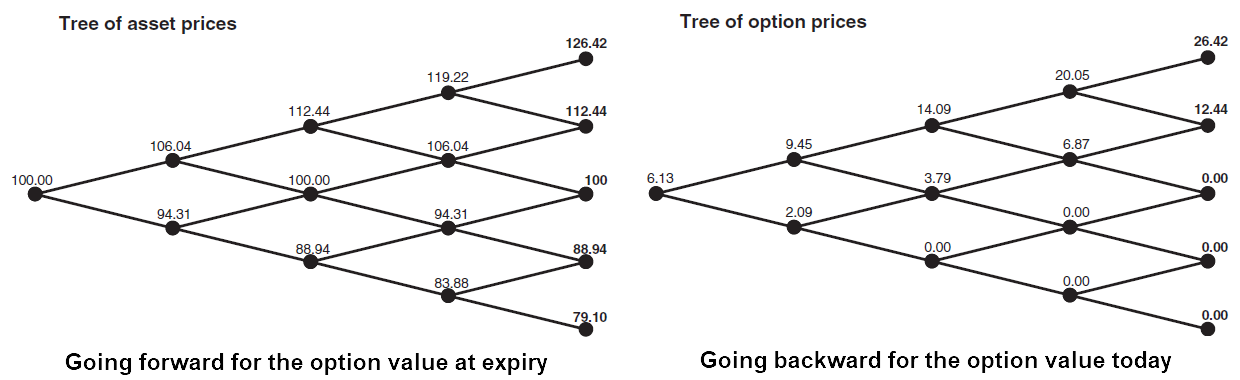
\includegraphics[width=\textwidth]{figure/binomial_tree.png} 
    \caption{The binomial tree}
    \label{fig:binomial_tree}
\end{figure}

The binomial tree also illustrate how to fully calculate the asset prices and the option prices. By going forward, one can find the option value at expiry $(V^+, V^-)$ at time $T$. As we know these values, we can find the option values one step further back in time. And by going backward to the root which is the current time and asset value, we can find the option value today. Programming of this process is given in Section \ref{sec:binomial_tree}

The aforementioned binomial setting is for European-style exercise. The algorithm of American-style exercise is identical with one exception  in the formula for $V$. We must ensure that there are no arbitrage opportunities at any of the nodes, i.e. the option value must be higher than the payoff value at any time.


\subsection{Miscellaneous}
The greeks are defined as derivatives of the option value with respect to various variables and parameters. These greeks will later be very important when we talk about risk management. It is important to distinguish whether the differentiation is with respect to a variable or a parameter (it could, of course, be with respect to both). If the differentiation is only with respect to the asset price and/or time then there is sufficient information in our binomial tree to estimate the derivative. It may not be an accurate estimate, but it will be an estimate. The option’s delta, gamma and theta, defined below can all be estimated from the tree. On the other hand, if you want to examine the sensitivity of the option with respect to one of the parameters, then you must perform another binomial calculation.

The binomial model can also lead us to the famous Black–Scholes equation. The binomial model is a discrete-time model whereas Black–Scholes is in continuous time.

The binomial method is just a simple version of an explicit finite-difference scheme. Finite-difference methods are far more flexible and can, in many ways, incorporate dividends, allow Bermudan exercise, value path-dependent contracts and price contracts depending on other stochastic variables such as interest rates. The binomial can also do these but in a more complicated way. 

Further remarks on risk neutrality by Paul Wilmott are given here:
\begin{itemize}
    \setlength\itemsep{0em}
    \item Hedging is used to eliminate risk.
    \item In simple models, hedging can be used to eliminate all risk from an option position.
    \item As well as eliminating risk, hedging removes dependence of an option value on the direction of an asset.
    \item If we don't care whether the asset price rises or falls, we shouldn't care about the probability of the rise or fall.
    \item \textit{The risk-neutral random walk is one that has the same volatility as the real asset random walk but a drift rate that is the same as the risk-free interest rate and not the real drift rate.}\footnote{Italic, here and down, means I still don't understand what Wilmott is talking about :).}
    \item \textit{The punchline is that the option value is the present value of the option payoff under a risk-neutral random walk}.
\end{itemize}



\section{Random behavior of assets}
\subsection{Jensen's inequality}
\textbf{Jensen's inequality}\index{Jensen's inequality} illustrates the importance of randomness in option theory. Let's look into the example below.

\begin{center}
\begin{footnotesize}
\fbox{
\begin{minipage}{0.90\textwidth}
The stock price is \$100 today. In one year's time, it could be \$50 or 150 with both equally likely. How can we value an option on this stock, e.g. a call option with a strike of 100 expiring in one year?

With those two possible scenarios we could say that we expect the stock price to be at \$100 in one year, this being the average of the possible future values. The payoff for the call option would then be 0, since it is exactly at the money. And the present value of this is zero.

Alternatively we could look at the two possible payoffs and then calculate that expectation. If the stock falls to 50 then the payoff is zero, if it rises to 150 then the payoff is 50. The average payoff is therefore 25, which we could present value to give us some idea of the option's value.

It turns out that the second calculation is closer to what we do in practice to value options although we know that the real probabilities don't come into the calculation. But that calculation illustrates another point of great importance, that the order in which we do the payoff calculation and the expectation matters, i.e.:
\begin{align}
    \text{Payoff} \left( \text{Expected} \left[ \text{Stock price} \right] \right) & = 0 \\
    \text{Expected} \left[ \text{Payoff} \left( \text{Stock price} \right) \right] & = 0     
\end{align}
This is an example of Jensen's inequality.

We can estimate how much the left-hand side is larger than the right-hand side. If we have a convex function $f(S)$ - the payoff function for a call of a random variable $S$ - the stock price then:
\begin{equation}
    E \left[ f \left( S \right) \right] \geq f \left( E \left[ S \right] \right)
\end{equation}

As $S$ is a random variable, let's assume that:
\begin{equation}
    S = E \left[ S \right] + \epsilon = \bar{S} + \epsilon
\end{equation}
in which $\bar{S}$ is the mean of $S$ and hence $E \left[ \epsilon \right] = 0$.

Now, we use the Taylor series approximation:
\begin{align}
    E \left[ f \left( S \right) \right] & = E \left[ f \! \left( \bar{S} + \epsilon \right) \right] = E \left[ f \! \left( \bar{S} \right) + \epsilon f' \! \left( \bar{S} \right) + \frac{1}{2} \epsilon^2 f'' \! \left( \bar{S} \right) \right] \\
    & \approx f \! \left( \bar{S} \right) + \frac{1}{2} f'' \! \left( \bar{S} \right) E \left[ \epsilon^2 \right] \\
    & = f \! \left[ E \left( S \right) \right] + \frac{1}{2} f'' \! \left( E \left[ S \right] \right) E \left[ \epsilon^2 \right]
\end{align}

$E \left[ \epsilon^2 \right]$ is the randomness in the underlying, and it variance. Modeling randomness is the key to modeling options.
\end{minipage}
}
\end{footnotesize}
\end{center}


\subsection{Returns}
This part is based on Chapter 4 of Wilmott \cite{pw_iqf2ed_2007}. When we invest in something, we would expect to have a comfortable return on our investment. By return, we mean the percentage growth in the value of an asset, together with accumulated dividends, over some period:
\begin{equation}
    \text{Return} = \frac{\text{change in value of the asset + accumulated cash flows}}{\text{original value of the asset}}
\end{equation}

When we model assets, it is the return that we should concentrate on. Part of the business of estimating returns for each asset is to estimate how much unpredictability there is in the asset value. It turns out that randomness plays a large part in financial markets \cite{pw_iqf2ed_2007}.

In modeling the returns, the following concepts, terms and processes are extremely important:
\begin{itemize}
    \setlength\itemsep{0em}
    \item The daily returns look very much like `noise' and is modeled as such. You, perhaps, have to wait months before you can spot the trend.
    \item The empirical returns are close enough to a random variable following the NORMAL distribution function with a non-zero mean and a non-zero standard deviation.
    \item The asset return model is similar to a model for a \textbf{random walk} of the asset price.
    \begin{equation}
        R_i = \frac{S_{i+1} - S_i}{S_i} = \mu \; \delta t + \sigma \; \phi \; \delta t^{1/2}
    \end{equation}
    or:
    \begin{equation}
        S_{i+1} = S_i \times \left(1 + \mu \; \delta t + \sigma \; \phi \; \delta t^{1/2} \right)
    \end{equation}    
    \item The parameter $\mu$ is called the drift rate, the expected return of the growth rate of the asset. In the classical option pricing theory, the drift plays almost no role. 
    \item The parameter $\sigma$ is called the volatility of the asset. The volatility is the most important and elusive quantity in the theory of derivatives. It is highly unlikely that volatility is constant for any given asset. Changing economic circumstances, seasonality, etc. will inevitably result in volatility changing with time.
    \item Because of their scaling with time, the drift and volatility have different effects on the asset path. The drift is not apparent over short timescales for which the volatility dominates. Over long timescales, for instance decades, the drift becomes important.
    \item The random walk model still have a discrete time step, this is a first step to develop a model in continuous-time. By changing from the normal distributions and discrete time to the \textbf{Wiener process}, the asset price model in the continuous-time limit using the Wiener process notation can be written as:
    \begin{equation}
        dS = \mu \; S \; dt + \sigma \; S \; dX
    \end{equation}
    This stochastic differential equation is a continuous-time model of an asset price. It is the most widely accepted model for equities, currencies, commodities and indices and the foundation of finance theory.
\end{itemize}
They will be described in more detailed in Section \ref{sec:randomness_assets}.